% !TeX encoding = UTF-8
% !TeX spellcheck = de_DE
% !TeX root = ./mainDoc.tex

\section{Anmerkungen zu ES6 Klassen und Vererbung} \label{keineKlassen}

Die meisten landläufig bekannten objektorientierte-Programmiersprachen (OO) basieren auf Klassen. 
%Klassisch: 
%- In klassischen OO-Sprachen wird zunächst eine Klasse als Blaupause definiert. 
%- Ein konkretes Objekt wird erzeugt indem eine "`Kopie"' dieser Blaupause materialisiert wird.
%- Es gibt kein Objekt ohne vorherige Klassendefinition.
In klassischen
%\footnote{Im Weiteren wird meist der Begriff \emph{klassisch} anstelle von \emph{klassenbasiert} verwendet, da in der englischsprachigen Literatur meist von \emph{classical} und nicht von \emph{class based} die Rede ist. Diese Begrifflichkeit soll hier übernommen werden.} 
OO-Sprachen wird für jedes Objekt zunächst eine Klasse definiert, die als Blaupause, bzw. abstraktes Modell für Objekte eines bestimmten Typs dient. Wenn nun ein konkretes Objekt --eine Instanz-- benötigt wird, so wird es anhand dieses vorher definierten Bauplans erstellt. Es handelt sich damit quasi um die "`materialisierte Kopie"' des Bauplans. In der klassischen Objektorientierung gibt es kein Objekt, zu dem nicht im Vorfeld eine Klasse definiert wurde. 

Ein weit verbreitetes Code-Reuse-Muster in klassischen Programmiersprachen ist die \emph{Vererbung}. Dabei werden Hierarchien von Klassen erstellt, deren Definitionen hierarchisch aufeinander aufbauen. Die in der Hierarchie weiter unten stehenden Klassen erben dabei Eigenschaften von Elternklassen, die weiter oben definiert wurden.

\begin{figure}[h]
	\centering
	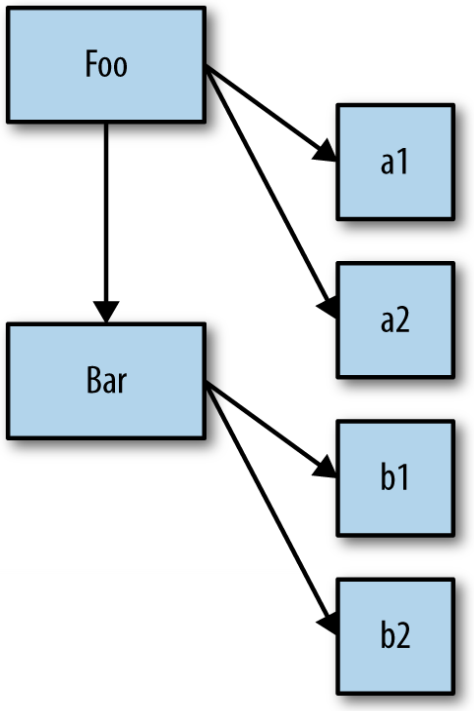
\includegraphics[width=0.3\textwidth]{images/classes_Simpson_p70.png}
	\caption{\label{classes}Vererbungshierarchie in einer klassischen OO-Sprache \\(aus \citep[p. 70]{SimpsonThisobjectprototypes2014}).}
\end{figure}

In Abbildung \ref{classes} ist eine solche (einfache) Hierarchie dargestellt. Ausgehend von der Klassendefinition \texttt{Foo} werden die beiden Objekte \texttt{a1} und \texttt{a2} instantiiert. Die Klasse \texttt{Bar} erbt alle Eigenschaften von \texttt{Foo} und kann eigene Spezialisierungen hinzufügen. Die konkreten Objekte \texttt{b1} und \texttt{b2} haben alle Fähigkeiten, die auch in der Klassendefinition \texttt{Foo} definiert wurden und haben zusätzlich noch weitere Eigenschaften, die in der Klassendefinition von \texttt{Bar} angegeben sind.

Diese Art der klassischen Objektorientierung ist seit ES6
%\footnote{
%ES6 steht für "`ECMAScript 6"'. \emph{ECMAScript} ist die offizielle Bezeichnung des Sprachstandards "`ECMA-262"', auf dem die als \emph{JavaScript} bezichneten Implementierungen beruhen. Im Folgenden wird weiter von JavaScript gesprochen, wenn allgemein die im Standard "`ECMA-262"' definierte Sprache gemeint ist. Wenn es um eine konkrete Version, oder eine Definition geht, so wird von ES\emph{x} gesprochen, wobei \emph{x} entweder eine Versionsnummer oder eine Jahreszahl ist. Zum Zeitpunkt der Erstellung (Winter 2018) ist  ES9 bzw. ES2018 die letzte Version des verabschiedeten Standards. (siehe \citep{international2018ecmascript})}
durch die Benutzung des Schlüsselwortes \texttt{class} auch in Javascript möglich. Es werden Klassen wie z. B. \texttt{class Foo \{\ldots \}} als Blaupausen definiert. Diese können mittels \texttt{class Bar extends Foo\{\ldots \}} zu klassischen Vererbungshierarchien ausgebaut werden. Damit lässt sich in Javascript sowohl syntaktisch als auch semantisch sehr ähnlich programmieren wie in klassischen OO-Sprachen.

\skippingparagraph

Im Kern ist JavaScript eine prototypenbasierte Programmiersprache, in der Objekte für sich alleine stehen und in der andere Techniken der Code-Wiederverwendung zur Verfügung stehen. Einige anerkannte Mitglieder der Javascript Community sind sogar der Meinung, dass die Einführung klassischer Sprachmittel eher nachteilig ist und damit mehr Probleme einhergehen als gelöst werden. Sie kritisieren die mit \texttt{class} eingeführte klassische Semantik in Javascript zum Teil heftig:

In \citep[p. 48ff. "`Classical Inheritance Is Obsolete"']{ElliottProgrammingJavaScriptapplications2014} führt Eric Elliot als Argumente gegen die klassische Vererbung u. a. an:
\begin{itemize}
	\item "`Tight Coupling"': Vererbung zwischen Klassen ist eine der engsten Kopplungen zwischen Komponenten, die in der Programmierung möglich ist. Die erbende Subklasse muss intime Kenntnisse der Implementierung der Basisklasse haben. Daraus ergibt sich direkt das \emph{Fragile Base Class Problem}, \citep[§6.2]{Steimann.2010}).
	\item "`Inflexible Hierarchies"': Nach einer Weile der Nutzung und bei steigender Benutzerbasis erweisen sich letztendlich sämtliche Klassenhierarchien als falsch, um bestimmte neue Nutzungsfälle damit zu modellieren. Durch die enge Kopplung ist es aber extrem schwierig bis unmöglich, diese Fehler durch Refactoring zu beheben.
	\item "`Gorilla/Banana Problem"': Die Vererbung läuft nach dem "`Alles oder Nichts"'-Prinzip und es ist nicht möglich nur einzelne Eigenschaften einer Basisklasse zu erben. Elliot zitiert \citep{SeibelCodersworkreflections2009}: \begin{quote}
	The problem with object-oriented languages is they’ve got all this implicit environment
	that they carry around with them. You wanted a banana but what you got was a gorilla
	holding the banana and the entire jungle.
	\end{quote}
	\item "`Duplicating by necessity"': Aufgrund der angesprochenen Probleme der klassischen Vererbung kommt es in vielen Applikationen dazu, dass entgegen aller Design-Prinzipien, Code Wiederverwendung durch Copy/Paste geschieht und damit der Idee der Vererbung zuwider läuft. 
\end{itemize}

Auch Douglas Crockford, Autor des Standardwerks "`JavaScript: the good parts"' (\citep{CrockfordJavaScriptgoodparts2008}) spricht sich letztendlich gegen klassische Vererbung in Javascript aus: \begin{quote}
I have been writing JavaScript for 14 years now, and I have never once found need to use an uber function. The super idea is fairly important in the classical pattern, but it appears to be unnecessary in the prototypal and functional patterns. I now see my early attempts to support the classical model in JavaScript as a mistake. \citep{CrockfordClassicalInheritanceJavaScript}
\end{quote}


Als letzter prominenten Vertreter der Kritiker sei hier noch Kyle Simpson erwähnt, der über die mit ES6-eingeführten Klassen in Javascript sagt:
\begin{quote}
Bottom line: if the ES6 \texttt{class} makes it harder to robustly leverage 
\texttt{[[Prototype]]}, and hides the most important nature of the JS object 
mechanism --the live delegation links between objects-- shouldn’t we 
see class as creating more troubles than it solves, and just relegate it
to an antipattern? \citep[p. 153]{SimpsonThisobjectprototypes2014}
\end{quote}

\skippingparagraph
Entsprechend dieser kritischen Einschätzung wurde in dieser Arbeit \emph{nicht} weiter auf die Möglichkeiten eingegangen, Javascript wie eine klassische OO-Sprache zu benutzen. 
%Die weiteren Betrachtungen konzentieren sich vielmehr darauf, was Javascript anders macht als klassische OO-Sprachen, und wie sich Javascript dadurch als einen Vertreter der prototypbasierten OO-Sprachen auszeichnet. 
Obwohl die mit ES6 eingeführten Klassen viele interessante Eigenschaften haben, ist es wichtig, Javascript zuerst als prototypenbasierte Sprache zu verstehen. Erst dann kann fundiert entschieden werden, welches Sprachmittel gewinnbringend eingesetzt werden soll.

Bei der für viele, aus anderen klassischen Sprachen kommende, Entwicklerinnen verlockenden Möglichkeit, über den ES6 \texttt{class}-Mechanismus auch JavaScript wie eine klassische Sprache zu benutzen, wird viel Potential verschwendet, das in der prototypischen und damit flexibleren Objektorientierung von JavaScript liegt.

Aus meiner Sicht ist es daher wichtig, vom prototypischen Ursprung von JavaScript aus zu denken und erst dann, wenn das nicht mehr ausreicht, die Erweiterungen zu betrachten, die der Sprache ein klassisches Gewand überstreifen. Andernfalls besteht die Gefahr, dass mit einen klassischen Hammer in der Hand jedes Problem aussieht wie ein Klassennagel.
